\documentclass[pdftex,11pt,a4paper,english,titlepage]{article}
\usepackage[utf8]{inputenc}
\usepackage[english]{babel}
\usepackage{color}
\usepackage{amsmath}
\usepackage{amsfonts}
\usepackage{amssymb}
\usepackage{natbib}
\usepackage{float}
\usepackage[pdftex]{graphicx}
\usepackage[left=1in,right=1in,top=1in,bottom=1in]{geometry}
\newcommand{\HRule}{\rule{\linewidth}{0.5mm}}

\author{Pieter Verlinden}
\title{Data Structures and Algorithms: Assignment 1}
\date{March 15, 2013}

\begin{document}

\begin{titlepage}
\begin{center}

\includegraphics[scale=0.25]{logo.jpg} \\
%
\includegraphics[scale=width=0.15\textwidth]{.logo.jpg}\\[1cm]
\textsc{\large Katholieke Universiteit Leuven}\\[4cm]
\textsc{\LARGE Data Structures and Algorithms}\\[0.5cm]

% Title
\HRule \\[0.4cm]
{ \huge \bfseries Assignment 1}\\[0.4cm]

\HRule \\[1.5cm]

%Author and lecturer
\begin{minipage}{0.45\textwidth}
\begin{flushleft} \large
\emph{Author:}
Pieter \textsc{Verlinden}\\

\emph{Student ID:}
r0369547\\

\emph{Study:}
1Ba Informatica

\end{flushleft}

\end{minipage}
\hfill
\begin{minipage}{0.45\textwidth}
\begin{flushleft} \large
\emph{Lecturer:} 
Dr.~Ir.~Philip \textsc{Dutré}
\end{flushleft}
\end{minipage}

\vfill

%bottom
{\large March 15, 2013}

\end{center}
\end{titlepage}
\tableofcontents
\newpage
\section{Introduction}
The purpose of this assignment is to study and compare a number of sorting algorithms. A conclusion will be made based on three experiments.\\

In the first experiment, four sorting algorithms (selection sort, insertion sort, mergesort and quicksort) are tested on their number of compares made to sort an array. Both sorted and unsorted arrays will be tested.

In the second experiment,\textit{{\color{red}TODO: write k-way}}\\
	
The last experiment is a double ratio experiment. This implies measuring the time for a sorting algorithm to sort an array of size $N$. Dividing the time to sort an array of size $2N$ with its previous time, gives us the doubling ratio of that algorithm.
In this experiment, insertion sort and quick sort will be tested and thoroughly discussed.
\section{Experiments}
		
	\subsection{Generic Sorting Algorithms}
This first experiment implies counting the compares made by each sorting algorithm. Methods for generating immense amounts of data input and data output gives us significant data which is then plotted in a scatter graph (see Figures \ref{fig:unsChart} and \ref{fig:sChart}).\\

One hundred arrays respectively with size $(0..N-1)$ and random values from $(0..N-1)$ were sorted. The amount of compares that each test returned are plotted on the chart in Figure \ref{fig:unsChart}.
As for the data in the chart in Figure \ref{fig:sChart}, the same method is maintained but with arrays that are already sorted.\\

\newpage
\textbf{Experimental data}\\
\begin{figure}[H]
	\centering
	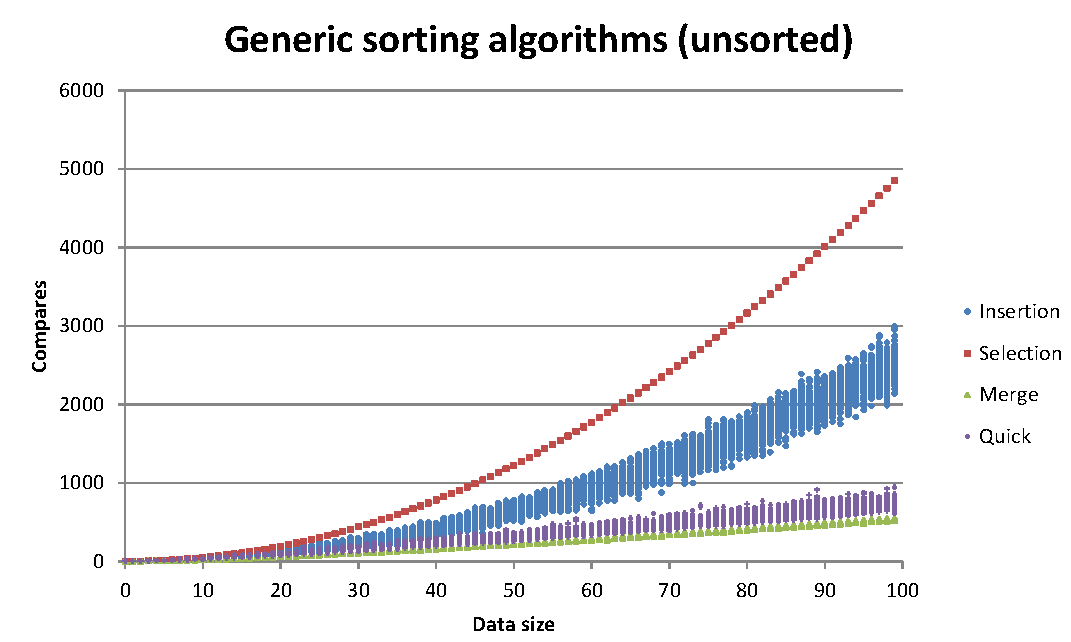
\includegraphics[scale=0.85]{unsortedChart.pdf} 
	\caption{Generic sorting algorithms data with unsorted arrays as input}
	\label{fig:unsChart}
\end{figure}

\begin{figure}[H]
	\centering
	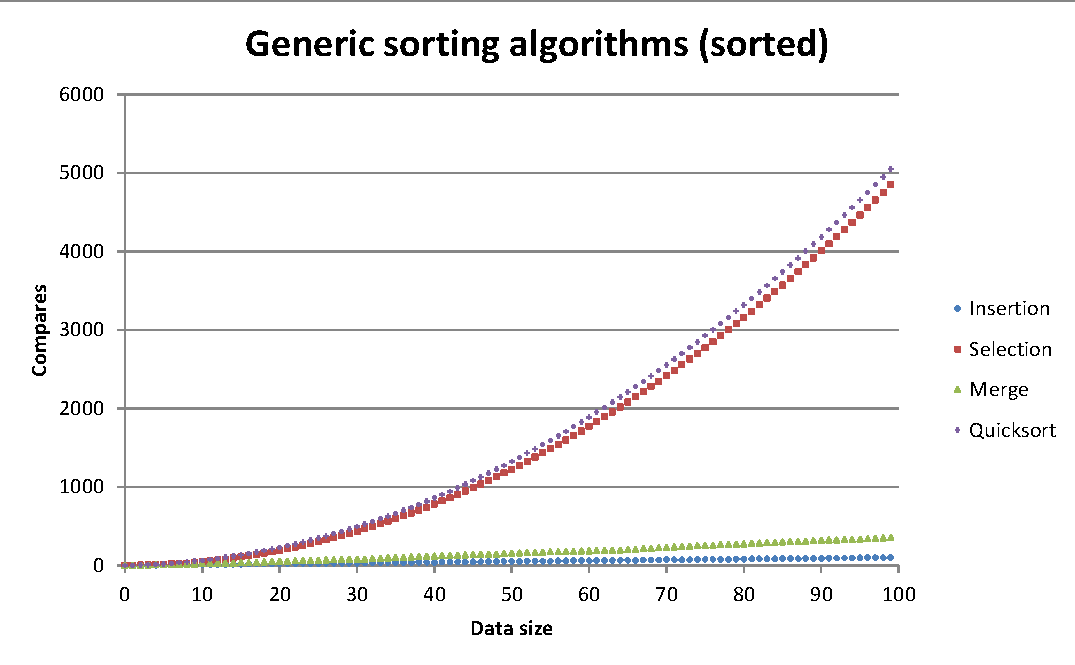
\includegraphics[scale=0.85]{sortedChart.pdf} 
	\caption{Generic sorting algorithms data with sorted arrays as input}
	\label{fig:sChart}
\end{figure}

    
		\subsubsection{Selection sort}
Selection sort works by selecting the smallest element in the array and exchanging it with the first entry then selecting the second smallest element and exchanging it with the second entry until the array is sorted.

\begin{quote}
\em \noindent \textbf{Proposition A.} Selection sort uses $\thicksim\frac{N^2}{2}$ compares and $N$ exchanges to sort an array of length $N$.\\
\tiny (Source: \citep{Sedgewick2011})
\end{quote}
As stated by proposition A, the expected compares of the selection sort algorithm proceeds according $$\thicksim\frac{N^2}{2}$$

Because selection sort checks every entry in an array, it is insensitive to input. This means that it takes about as long to run selection sort for an array that is sorted or for an array with all values equal as it does for an array with random elements.\\

As we can see in Figure \ref{fig:unsChart}, the compares of selection sort (red dotted line) grow quadratically. Because there are no values surrounding the line (like the thick dotted line of the compares of insertion) we can conclude that selection sort is insensitive to input. The data in Figure \ref{fig:sChart} confirms our statement of insensitivity by the fact that there is no difference between the compares of an array with random values or between the compares of an array with sorted values.

		\subsubsection{Insertion sort}\label{sec:insertion}
Insertion sort works by inserting elements according to their size in the array. The items at the left side are in order during the sort, however they are not in their final position. They may have to be moved so other elements can be inserted.

\begin{quote}
\em \noindent \textbf{Proposition B.} Insertion sort uses $\thicksim\frac{N^2}{4}$ and $\thicksim\frac{N^2}{4}$ exchanges to sort a randomly ordered array of length N with distinct keys, on the average. The worst case is $\thicksim\frac{N^2}{2}$ compares and $\thicksim\frac{N^2}{2}$ exchanges and the best case is $N-1$ compares and $0$ exchanges.\\
\tiny (Source: \cite{Sedgewick2011})
\end{quote}

As stated by proposition B, the expected compares and exchanges proceeds according $$\thicksim\frac{N^2}{4}$$

The insertion sort algorithm is very input sensitive. In Figure \ref{fig:unsChart} we see that insertion sort has the most spread data which proves our theorem true.
From the data in Figure \ref{fig:sChart} we can conclude that the insertion sort algorithm is the most efficient for sorted and nearly sorted arrays. 

		\subsubsection{Mergesort}
Mergesort is a recursive sorting algorithm based on the principle of splitting, sorting and merging. An array is recursively split until only auxiliary arrays of length one remain. Each auxiliary array then sorts and merges itself until the original array is sorted.

\begin{quote}
\em \noindent \textbf{Proposition F.} Top-down mergesort uses between $\frac{1}{2}N\log N$ and $N\log N$ compares to sort an array of length N.\\
\tiny (Source: \cite{Sedgewick2011})
\end{quote}

As stated by proposition F, the expected compares proceeds according $$\thicksim N\log N$$

One of the great advantages of mergesort is that it offers certainty about the time to sort. If we sort an array of size N, the time that is needed to sort this array will always be proportional to $N\log N$. One major let-down is the extra use of space proportional to N.

As we can see in Figure \ref{fig:unsChart} and Figure \ref{fig:sChart}, mergesort is a very time-stable algorithm and is not very sensitive to input. According to our results we could state that mergesort is the most efficient algorithm. However, the extra space that is needed makes it extensively slower due to memory access time.

		\subsubsection{Quicksort}\label{sec:quick}
Quicksort is also a recursive sorting algorithm based on partitioning an array into two subarrays. The two subarrays will then be sorted independently. It has many in common with mergesort where we break the array into two subarrays, sort and merge them. Quicksort splits the array in two subarrays of different length. the position where the array is split depends on the contents of the array.\\
The major advantage of quicksort is that, unlike mergesort, it uses far less space and makes it superior to the mergesort algorithm.

\begin{quote}
\em \noindent \textbf{Proposition K.} Quicksort uses $\thicksim 2N\log N$ compares (and one-sixth that many exchanges) on the average to sort an array of length N with distinct keys.\\
\tiny (Source: \cite{Sedgewick2011})
\end{quote}

\begin{quote}
\em \noindent \textbf{Proposition L.} Quicksort uses $\thicksim\frac{N^2}{2}$ compares in the worst case, but random shuffling protects against this case.\\
\tiny (Source: \cite{Sedgewick2011})
\end{quote}
As stated by proposition K the expected compares proceeds according $$\thicksim 2N\log N$$

The data in Figure \ref{fig:sChart} confirms proposition L. An array that is already sorted is the worst case scenario for the used quicksort algorithm. This is due to the chose of pivot point. In the used algorithm, the first entry is chosen as pivot. As the array is already sorted, the first element will always be the smallest one which leads to a recursive call on whole the array minus one element. This will lead to a very inefficient algorithm. A random shuffle of the elements in the array protects against this occurrence. Since an array with random elements can be represented by a shuffled array, Figure \ref{fig:unsChart} proves the shuffle theorem true.

	\subsection{K-way Merge Sort}
		//TODO: write report on k-way merge sort experiment
		
	\subsection{Doubling ratio experiment}
In this experiment, actual time will be measured to determine a certain ratio. This report only tests two of five algorithms, insertion sort and quicksort.

		\subsubsection{Insertion sort}\label{sec:insDR}
\begin{table}[H]
	\centering
	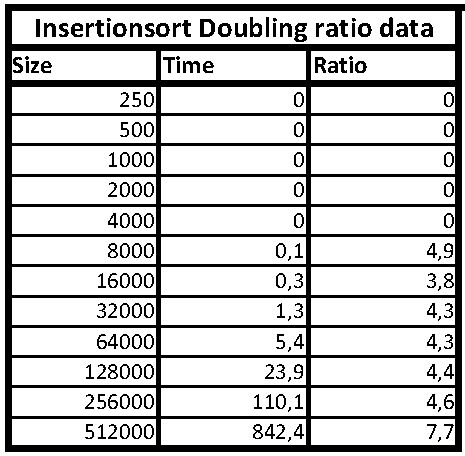
\includegraphics[scale=1]{insertionDRdata.pdf}
	\caption{Doubling ratio data for insertion sort.\label{tab:insDRdata}}
\end{table}

From the data listed in Table \ref{tab:insDRdata}, we can conclude that the insertion sort algorithm has a doubling ratio value of $\pm$4.\\
In the last row, the doubling ratio value is 7,7. This is due to the large amount of time the algorithm needs to sort an array of this size. If the process of sorting is interrupted by other processes running on the computer, the amount of time could increase extensively.\\

Section \ref{sec:insertion} states that the compares of insertion sort grow according $\thicksim\frac{N^2}{4}$. From this point we can derive the doubling ratio. $$\frac{(2N)^2}{4}=\frac{4N^2}{4}=N^2$$
$$\text{ratio: } \frac{N^2}{\frac{N^2}{4}}=\frac{4N^2}{N^2}=4$$

With this ratio we can predict the time needed to sort an array of size $2N$. e.g. the time needed to sort an array of size $512'000$ according to the time for sorting an array of size $256'000$, is $110s*4 = 440s$ (see Table \ref{tab:insDRdata}). This is significantly lower then the real sorting time but this is due to the fact stated above.

		\subsubsection{Quicksort}
\begin{table}[H]
	\centering
	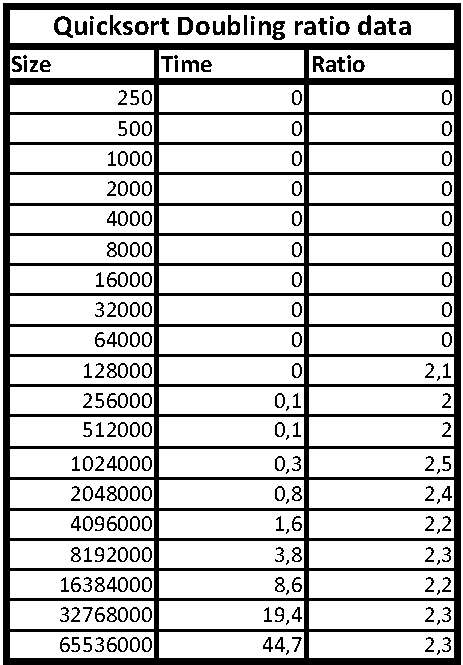
\includegraphics[scale=1]{quickDRdata.pdf}
	\caption{Doubling ratio data for quicksort.\label{tab:quickDRdata}}
\end{table}

From the data listed in Table \ref{tab:quickDRdata}, we can conclude that the quicksort algorithm has a doubling ratio value of $\pm$2.\\

Section \ref{sec:quick} states that the compares of quicksort grow according $\thicksim 2N\log N$. We apply the same method for deriving the doubling ratio as used in section \ref{sec:insDR}. $$2(2N)\log (2N)=4N(\log N + \log 2)$$
$$\text{ratio: } \frac{4N(\log N + \log 2)}{2N\log N} = 2*(\frac{\log 2}{\log N} + 1)= \frac{\log 4}{\log N}+2$$
$$\Downarrow$$  
$$\lim_{N \to +\infty}(\frac{\log 4}{\log N}+2) = 2$$

Again we can predict the time needed to sort an array of size $2N$. e.g. the time needed to sort an array of size $131'072'000$, is $44{,}7s*2 = 89{,}4s$ (see Table \ref{tab:quickDRdata}).

\newpage
\bibliographystyle{plain}
\bibliography{bibTeX}
\end{document}


